\chapter{Hiện thực nhận dữ liệu cho gateway}
\section{Giới thiệu}
Sử dụng công nghệ truyền thông không dây LoRa \cite{tl12} (Long Range Radio) và nền tảng Android Things cho gateway.
\begin{center}
\begin{figure}[htp]
\begin{center}
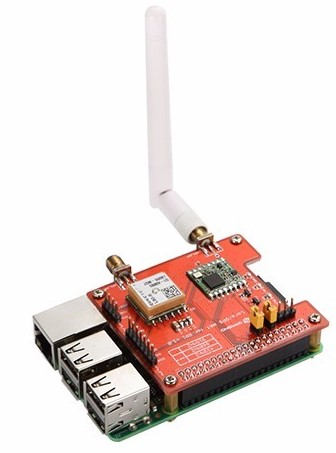
\includegraphics[scale=0.55]{image5/lorahat.jpg}
\end{center}
\caption{Gateway LoRa}
\end{figure}
\end{center}
\subsection{LoRa}
\textit{Xem thêm \hyperref[chapterlora]{LoRa - Mục \ref{chapterlora}}}

\subsection{Android Things}
\textit{Xem thêm \hyperref[chapter3]{Chương 3}}

\section{Phát triển driver cho gateway: SPI}
\subsection{Giới thiệu SPI}
SPI viết tắt của Serial Peripheral Interface \cite{tl10}, SPI bus – Giao diện ngoại vi nói tiếp, bus SPI. Chuẩn SPI được phát triển bởi Motorola. Đây là một chuẩn đồng bộ nối tiếp để truyền dữ liệu ở chế độ song công toàn phần (full- duplex) tức trong cùng một thời điểm có thể xảy ra đồng thời quá trình truyền và nhận. Đôi khi SPI còn được gọi là chuẩn giao tiếp 4 dây (Four-wire).\\
SPI là giao diện đồng bộ, bất cứ quá trình truyền nào cũng được đồng bộ hóa với tín hiệu clock chung. Tín hiệu này sinh ra bởi master.\\
\begin{figure}[htp]
\begin{center}
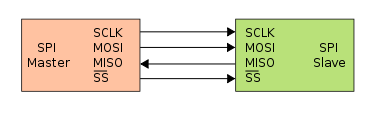
\includegraphics[scale=1]{image5/khainiem.png}
\end{center}
\caption{Khái niệm SPI}
\end{figure}
Trong giao diện SPI có bốn tín hiệu số:
\begin{itemize}
\item MOSI hay SI – cổng ra của bên Master ( Master Out Slave IN). Đây là chân dành cho việc truyền tín hiệu từ thiết bị chủ động đến thiết bị bị động.
\item MISO hay SO – Công ra bên Slave (Master IN Slave Out). Đây là chân dành cho việc truyền dữ liệu từ Slave đến Master.
\item SCLK hay SCK là tín hiệu clock đồng bộ (Serial Clock). Xung nhịp chỉ được tạo bởi Master.
\item CS hay SS là tín hiệu chọn vi mạch ( Chip Select hoặc Slave Select). SS sẽ ở mức cao khi không làm việc. Nếu Master kéo SS xuông thấp thì sẽ xảy ra quá trình giao tiếp. Chỉ có một đường SS trên mỗi slave nhưng có thể có nhiều đường điều khiển SS trên master, tùy thuộc vào thiết kế của người dùng.
\end{itemize}
\begin{figure}[htp]
\begin{center}
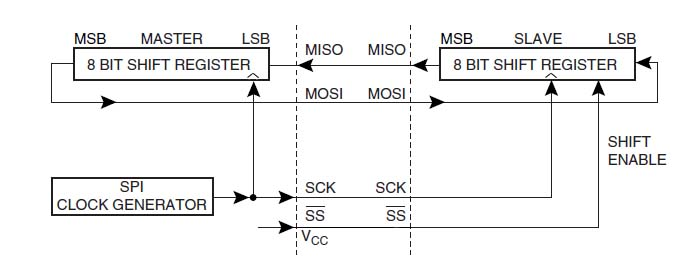
\includegraphics[scale=0.6]{image5/nguyenly3.jpg}
\end{center}
\caption{Sơ đồ đường đi của SPI}
\end{figure}
\newpage
\subsection{Nguyên lý hoạt động}
Để bắt đầu hoạt động thì kéo chân SS xuống thấp và kích hoạt clock ở cả Maser và Slave.
\begin{center}
\begin{figure}[htp]
\begin{center}
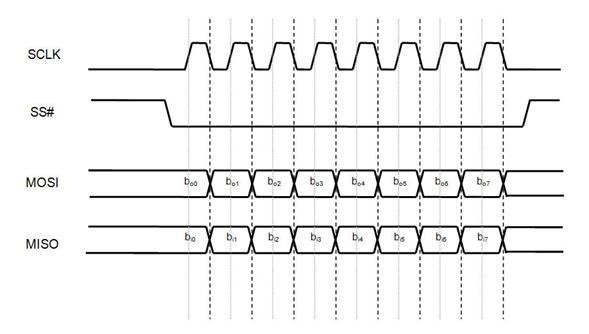
\includegraphics[scale=1]{image5/nguyenly1.jpg}
\end{center}
\caption{Nguyên lý hoạt động của SPI}
\end{figure}
\end{center}
Mỗi chip Master hay Slave có một thanh ghi dữ liệu 8 bits.\\
Cứ mỗi của xung nhịp do Master tạo ra trên đường giữ nhịp SCK, một bit trong thanh ghi dữ liệu của Master được truyền qua Slave trên đường MOSI, đồng thời một bit trong thanh ghi dữ liệu của chip Slave cũng được truyền qua Master trên đường MISO.\\
Lưu ý, có thể config tín hiệu đồng bộ clock theo sườn, theo mức ….\\
Hiện tại có 4 mode cơ bản (MODE 0. 1,2,3) của SPI dựa vào config SCLK như sau:\\
\begin{center}
\begin{figure}[htp]
\begin{center}
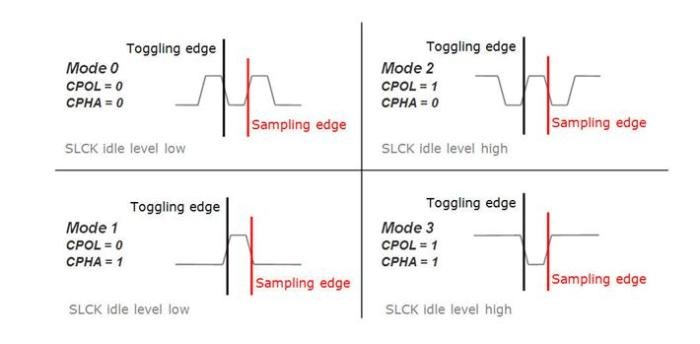
\includegraphics[scale=1]{image5/nguyenly2.jpg}
\end{center}
\caption{Dạng sóng của 4 mode SPI}
\end{figure}
\end{center}
\newpage
Cực của xung giữ nhịp, phase và các chế độ hoạt động: cực của xung giữ nhịp (Clock Polarity) được gọi tắt là CPOL .Đây là khái niệm dùng chỉ trạng thái của chân SCK ở trạng thái nghỉ.\\
Ở trạng thái nghỉ (Idle), chân SCK có thể được giữ ở mức cao (CPOL=1) hoặc thấp (CPOL=0).\\
Phase (CPHA) dùng để chỉ cách mà dữ liệu được lấy mẫu (sample) theo xung giữ nhịp.\\
Dữ liệu có thể được lấy mẫu ở cạnh lên của SCK (CPHA=0) hoặc cạnh xuống (CPHA=1).\\

\begin{table}[!h]
\begin{center}
\begin{tabular}{|c|c|c|}
\hline
\textbf{SPI Mode} & \textbf{SCK (Cạnh bắt đầu)} & \textbf{SCK (Cạnh kết thúc)} \\ 
\hline
0 & Lấy mẫu dữ liệu tại cạnh lên & Truyền dữ liệu mới tại cạnh xuống\\
\hline
1 & Truyền dữ liệu mới tại cạnh lên & Lấy mẫu dữ liệu tại cạnh xuống\\
\hline
2 & Lấy mẫu dữ liệu tại cạnh xuống & Truyền dữ liệu mới tại cạnh lên\\
\hline
3 & Truyền dữ liệu mới tại cạnh xuống & Lấy mẫu dữ liệu tại cạnh lên\\
\hline
\end{tabular}
\caption{Các mode trong giao tiếp SPI \cite{tl11}}
\end{center}
\end{table}

\subsection{Driver SPI của Raspberry Pi 3 và LoRa HAT}
Sử dụng ngôn ngữ JAVA đễ thiết kế Driver SPI trên nền tảng Andoird Things.
\subsubsection{Cấu hình kết nối SPI}
Dựa vào \href{https://www.mouser.com/ds/2/761/sx1276-944191.pdf}{Datasheet LoRa}  của SEMTECH, có thể xác định được các thông số sau:
\begin{itemize}
    \item SPI Mode: MODE 1.
    \item SPI Frequency: 32,000,000Hz (32MHz).
    \item SPI First Bit: Bit MSB - bit có trọng số cao.
    \item SPI Bits Per Word: 8 bits.
\end{itemize}
\begin{lstlisting}[label={list:first},caption=Cấu hình SPI cho việc giao tiếp]
void configSPIDevice(SpiDevice device) throws IOException {
    device.setMode(SpiDevice.MODE1);
    device.setFrequency(32000000); // 32MHz
    device.setBitJustification(SpiDevice.BIT_JUSTIFICATION_MSB_FIRST);
    device.setBitsPerWord(8);
    Log.d(TAG,"SPI OK now ....");
}
\end{lstlisting}
\subsubsection{Khởi động giao tiếp giữa LoRa và Rpi3}
Đầu tiên, cần chạy lệnh \lstinline{begin();}.
\begin{enumerate}
\item Tín hiệu tại chân RESET tích cực thấp để thiết lập giá trị của các thanh ghi về 0x00.
\item Sau đó sẽ đưa LoRa vào trạng thái ngủ (Sleep mode: 0x00) để tiến hành thiết lập các thông số cần thiết.\vspace*{0.5cm}\\
\textit{Việc thiết lập trạng thái hoạt động của LoRa phải thực hiện lệnh GHI (\lstinline{writeRegister()}) lên thanh ghi REG\_OP\_MODE, địa chỉ 0x01.}
\item Thiết lập tần số hoạt động (thường dùng 434MHz), giá trị thanh ghi TX (gửi), RX (nhận) về 0x00, năng lượng truyền (thường dùng 13dBm),...
\item Sau khi thiết lập xong, chuyển LoRa vào trạng thái chờ (chuẩn bị hoạt động - Standby mode: 0x01).
\end{enumerate}
\begin{lstlisting}[label={list:second},caption=Khởi động việc điều khiển board LoRa]
public int begin(long frequency) throws IOException {

    // perform reset
    digitalWrite(pinReset, LOW);
    delay(10);
    digitalWrite(pinReset, HIGH);
    delay(10);

    // start SPI
    configSPIDevice(mDevice);

    // check version
    byte version = readRegister(REG_VERSION);
    if (version != 0x12) {
        return 0;
    }

    // put in sleep mode to set LoRa mode
    sleep();

    // set frequency, usually 434MHz
    setFrequency(frequency);

    // set base addresses
    writeRegister(REG_FIFO_TX_BASE_ADDR, (byte) 0);
    writeRegister(REG_FIFO_RX_BASE_ADDR, (byte) 0);

    // set LNA boost
    writeRegister(REG_LNA, (byte) (readRegister(REG_LNA) | 0x03));

    // set auto AGC
    writeRegister(REG_MODEM_CONFIG_3, (byte) 0x04);

    // set output power to 17 dBm
    setTxPower(13, PA_OUTPUT_PA_BOOST_PIN);

    // put in standby mode to start working
    idle();

    return 1;
}
\end{lstlisting}

Để gửi gói tin, dùng lệnh \lstinline{LoRaSender(string);}.
\begin{enumerate}
\item Đầu tiên, LoRa sẽ kiểm tra có đang trong trạng thái gửi gói tin nào không. Nếu không thì một gói tin mới sẽ được tạo ra với kích thước là 0 (REG\_PAYLOAD\_LENGTH = 0x00).
\item Nội dung cần được gửi đi sẽ thêm vào gói tin vừa được tạo bằng lệnh \lstinline{write(string)}.
\item LoRa chuyển sang chế độ gửi tin (MODE\_TX: 0x03). Gói tin được gửi đi. LoRa sẽ chờ cho đến khi gói tin hoàn toàn gửi xong mới kết thúc quá trình gửi.
\end{enumerate}
\begin{lstlisting}[label={list:third},caption=Hàm gửi gói tin]
public void LoRaSender(String string){
    beginPacket(0);
    write(string.getBytes());
    endPacket(false);
    delay(5000);
}
\end{lstlisting}

Để nhận gói tin, dùng lệnh \lstinline{LoRaReceive();}.
\begin{enumerate}
\item Hàm \lstinline{parsePacket()} sẽ chuyển LoRa về chế độ nhận gói tin \newline(MODE\_RX\_SINGLE: 0x06).
\item Nếu có tin hiệu của gói tin đang được gửi đến (thường là Header), tiếp tục chuyển sang chế độ MODE\_RX\_CONTINOUS: 0x05 để nhận tất cả phần còn lại của gói tin.
\item Toàn bộ dữ liệu của gói tin vừa nhận được lưu ở thanh ghi REG\_FIFO (địa chỉ 0x00). Nội dung sẽ được đọc lên bởi lệnh \lstinline{read()}, dữ liệu được lưu ở dạng "byte" nên cần phải dùng kiểu "char" để chuyển thành ngôn ngữ bình thường.
\end{enumerate}
\begin{lstlisting}[label={list:fourth},caption=Hàm nhận gói tin]
public void LoRaReceive(){
    int packetSize = parsePacket(0);
    if (packetSize > 0) {
        String dataTemp = "";
        // received a packet
        dataTemp += "Received packet '";
        // read packet
        while (available() > 0) {
            dataTemp += (char)read();
        }
        // print string
        Log.d(TAG,dataTemp);
    }
}
\end{lstlisting}

Khi không cần sử dụng nữa, chỉ cần dùng lệnh \lstinline{end();} để ngắt kết nối giao tiếp SPI giữa mạch Rpi3 và LoRa HAT.
\begin{lstlisting}[label={list:fifth},caption=Kết thúc việc điều khiển board LoRa]
public void end(){
    if (mDevice != null) {
        try {
            mDevice.close();
            mDevice = null;
        } catch (IOException e) {
            Log.w(TAG, "Unable to close SPI device", e);
        }
    }
}
\end{lstlisting}

\href{https://github.com/phuongnam0907/ConfigLoRa}{[GITHUB] https://github.com/phuongnam0907/ConfigLoRa} 
%
%
%\section{Xây dựng chương trình nhận dữ liệu}
%
%
%\section{Xây dựng chương trình gửi dữ liệu lên Cloud}
%
%